\documentclass{beamer}
\usepackage{tikz}
\usetikzlibrary{trees,arrows}

\usetheme{CMU}

\title{AutoMerge}
\subtitle{}
\date{\today}
\author[Fonseca Mesner]{Francisco Fonseca \and Octavio Mesner}
\institute{Carnegie Mellon University}

\begin{document}
\maketitle

%\section{}
%\begin{frame}
%\frametitle{Goals}
%Discuss
%\begin{itemize}
%\item Outline Problem
%\item Alternatives
%\item Explain Costs and Calculations
%\item Specify Uncertainty
%\item State Assumptions
%\item Show Results
%\item Convey Sensitivity Analyses
%\item Conclusion
%\end{itemize}
%\end{frame}

\section{Problem}

\begin{frame}
  \frametitle{Problem}
  \framesubtitle{Overview}
  \begin{itemize}
  \item NYC to become a leader in \emph{smart city} infrastructure
  \item One piece: Evaluate autononous vehicles
  \item By 2020, NYC expects its fleet to be autonomous.
  \item We will evaluate AutoMerge (AM) Inc as an alternative.
  \end{itemize}
\end{frame}

\section{Alternatives}
\begin{frame}
  \frametitle{Alternatives}
  \begin{enumerate}
  \item Do not not implement AM.\\
    This are the costs that would be incurred if the status quo
    continues so there is little uncertainty for this alternative.
  \item Implement AM.\\
    Implementing AM comes with uncertainty with respect to AM
    performance.
  \item Perform a pilot study.\\
    We decide size of pilot study.  A larger the study reduces more
    uncertainty than a smaller one but costs more.
  \end{enumerate}
\end{frame}

\section{Costs and Calculations}
\begin{frame}
  \frametitle{Costs and Calculations}
  \begin{table}[h]
%\caption{Capital and O\&M costs of the AM system}
\centering
\tiny
\renewcommand{\arraystretch}{1.1}
\begin{tabular}{c l l l}
\hline
 	& Variable 							& Value 				& Notes 						\\\hline\hline
(a)	& \# buses with age $<$ 5 years				& 2313				& Source:	 \cite{am1}	\\
(b)	& \# buses with age 5-9 years				& 1296				& Source:	\cite{am1}					\\
(c)	& \# buses with age 10-20 years			& 1437				& Source:	\cite{am1}					\\
(d)	& Capital Cost per bus age $<$ 5 years		& \$ 5000				& Source:	\cite{am1}		\\
(e)	& Capital Cost per bus age 5-9 years		& \$ 6500				& Source:	\cite{am1}		\\
(f)	& Capital Cost per bus age 10-20 years		& \$ 8500				& Source:	\cite{am1}		\\
\textbf{(g)}	& \textbf{Total Capital Cost}(*)			& \textbf{\$ 45.7 Million}	& \textbf{=(a)*(d)+(b)*(e)+(c)*(f)}			\\
(h)	& Annual O\&M Cost per Bus				& \$ 1500				& Source:	\cite{am1}	\\
\textbf{(i)}	& \textbf{Total Annual O\&M Cost} (**)	& \textbf{\$
  7.6 Million}	& \textbf{=[(a)+(b)+(c)]*(h)}\\
(j)	& Annual Cost per Commuter				& \$ 1739				& Source:	\cite{UMR}	\\
(k)	& Annual hours in congestion per commuter	& 74 hours			& Source:	\cite{UMR} 	\\
(l)	& Cost per minute 						& \$ 0.39				& $(h)/[(i)*60]$		\\
(m)	& Total person trip per day					& 1.52 million			& Source: 	\cite{nyctransit}	\\
(n)	& Average time in daily person trip			& 49 minutes			& Source:	\cite{nyctransit}	\\
\textbf{(o)}	& \textbf{Total annual congestion cost}	& \textbf{\$ 10.5 Billion}	& \textbf{=360*(l*(k)*(j)}			\\\hline\hline
%\multicolumn{4}{l}{{\footnotesize (*) Capital costs are considered to be incurred only in the first year}} \\
%\multicolumn{4}{l}{{\footnotesize (**) O\&M costs begin to occur in the fifth year of the analysis (when AM starts operating)}} \\
\end{tabular}
%\label{tab:am.cost}
\end{table}%
\end{frame}

\section{Uncertainty}
\begin{frame}
  \frametitle{Uncertainty}
  \begin{columns}
    \begin{column}{0.4\textwidth}
      We account for uncertainty using decision trees.  Our sources of
      uncertainty are weather and proformance of AM.
    \end{column}
    \begin{column}{0.6\textwidth}
      \centering
      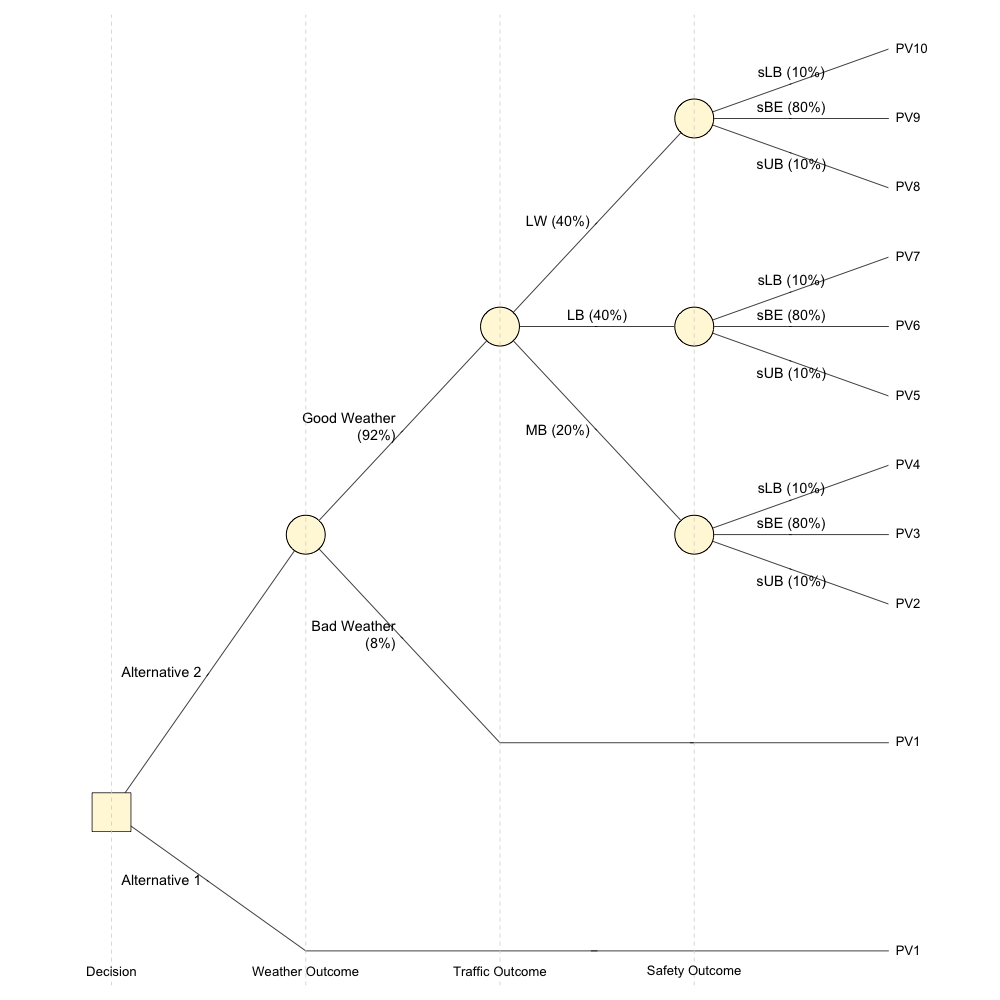
\includegraphics[width=\textwidth]{../../R/decisiontree}
    \end{column}
  \end{columns}
\end{frame}

\section{Assumptions}
\begin{frame}
  \frametitle{Assumptions}
\end{frame}

\section{Pilot Study}
\begin{frame}
  \frametitle{Pilot}
  \begin{columns}
    \begin{column}{0.4\textwidth}
      \begin{itemize}
      \item Uses EVII and Bayes Theorem to compute
      \item Figure shows value study after associated cost.
      \item Optimum value from 100\% of fleet.
      \end{itemize}
    \end{column}
    \begin{column}{0.6\textwidth}
      \centering
      \includegraphics[width=\textwidth]{../../R/alt3barplot}
    \end{column}
  \end{columns}
\end{frame}

\section{Results}
\begin{frame}
  \frametitle{Results}

  \centering
  %\includegraphics[width=0.9\textwidth]{10foldCv}
\end{frame}

\section{Sensitivity}
\begin{frame}
  \frametitle{Sensitivity Analyses}
  \begin{columns}
    \begin{column}{0.35\textwidth}
      \begin{itemize}
      \item Input values varied between 50 and 200\% or more. 
      \item Dashed line indicates baseline assumption
      \item Discount rate, VSL, and per person cost of commute time
        all greatly affect net expected cost but similarly for all.
      \item Weather affects alternatives 2 and 3 more then 1 but
        alternative 1 remained more expensive.
      \end{itemize}
    \end{column}
    \begin{column}{0.65\textwidth}
      \centering
      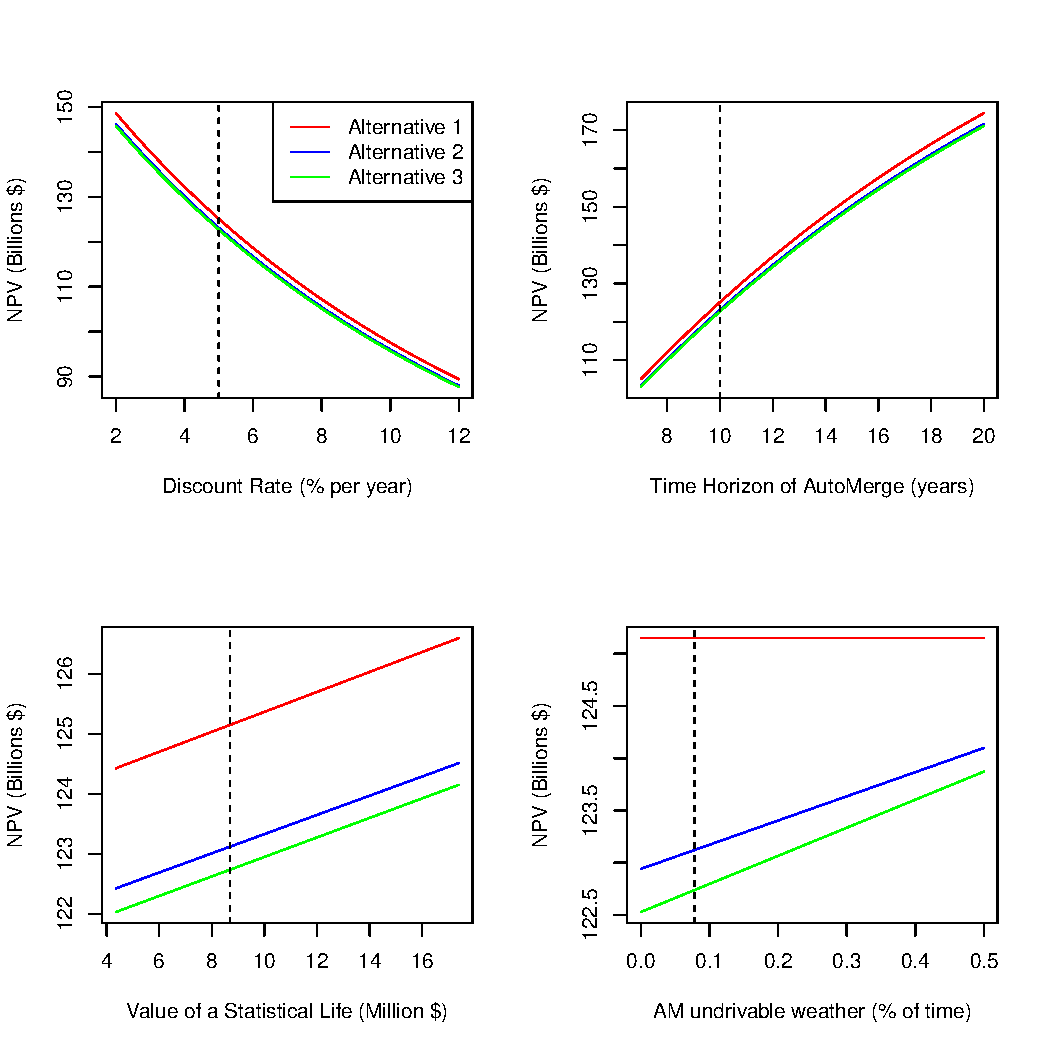
\includegraphics[width=\textwidth]{../../R/sensitivity}
    \end{column}
  \end{columns}
\end{frame}

\section{Conclusion}
\begin{frame}
  \frametitle{Conclusion}
  \begin{itemize}
  \item
  \end{itemize}
\end{frame}


\section{References}
\begin{frame}
  \frametitle{References}
  \bibliography{../report/bibfile.bib}{}
  \bibliographystyle{plain}
\end{frame}

\end{document}
